% Звіт
% • Титульна сторінка
% • Опис хромосоми
% • Опис обраних варіантів схрещування та мутації
% • Опис головних гіперпараметрів та їх значення (розмір популяції, елітизм, ...) для кожного експерименту, графічні результати
% • Опис експериментів для кожної функції
% • Висновки
% • До звіту бажано додати (окремим файлом) анімаційне зображення процесу пошуку.

\documentclass{article}
\usepackage{graphicx}
\usepackage{epstopdf}
\usepackage{lipsum}
\usepackage[T2A]{fontenc}
\usepackage[utf8]{inputenc}

\graphicspath{ {../Images/} }

\epstopdfDeclareGraphicsRule{.gif}{png}{.png}{convert gif:#1 png:\OutputFile}
\AppendGraphicsExtensions{.gif}

\begin{document}
    \begin{titlepage}
        \begin{center}
        $\newline$
        \vspace{3.3cm}
        
        {\LARGE\textbf{Лабораторна робота №1\\"Розробка програмного забезпечення для розв’язання оптимізаційних задач за допомогою генетичних алгоритмів"}}
        \vspace{10cm}
        \begin{flushright}
            \textbf{Роботу виконав:}\\Климентьєв Максим \\3-го курсу\\групи ФІ-21
        \end{flushright}
        \end{center}
    \end{titlepage}
    \newpage

    \tableofcontents 
    \section{Опис хромосоми}
        \textbf{Хромосома} --- число обране за допомогою рівномірного розподілу на заданому проміжку
    \section{Опис обраних варіантів схрещування та мутації}
        \textbf{Схрещування} --- число, обране за допомогою рівномірного розподілу на відрізку між мінімальним та максимальним серед батьків
        \textbf{Мутація} --- число обране за допомогою рівномірного розподілу на заданому проміжку

    \section{Опис головних гіперпараметрів та їх значення (розмір популяції, елітизм, ...) для кожного експерименту, графічні результати}
        \textbf{Розмір популяції} --- найкращі, які потім схрещуються і створюють нову, більш кращу популяцію
        \textbf{Кількість схрещувань} --- чим більше значення, тим більше "дітей" буде утворюватися з минулої популяції
        \textbf{Ймовірність мутації} --- ймовірність, що "дитина" може взагалі не походити на батька, бути гірше, або навіть краще.

    \section{Опис експериментів для кожної функції}
        \textbf{Вони були однакові} --- Для кожної функції було проведено по 3 експерименти:
        \begin{enumerate}
            \item Коли розмір популяції великий
            \item Коли кількість схрещувань велика
            \item Коли 100\% ймовірність мутації
        \end{enumerate}

    \newpage
    \section{Висновки}
        \textbf{Branin Function} --- найкраще вийшло, коли кількість схрещувань велика \\
        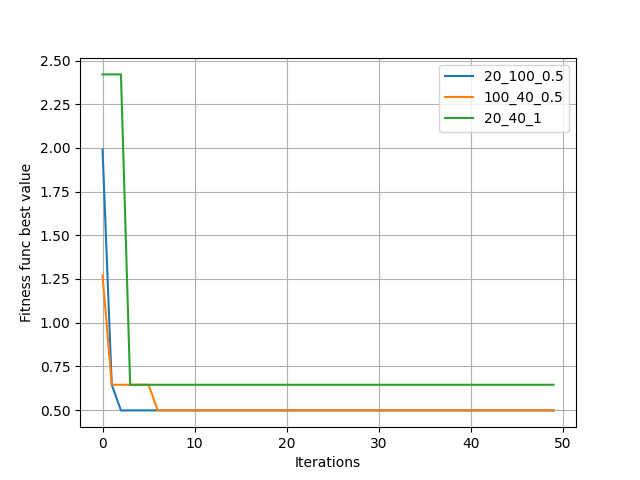
\includegraphics{Branin Function.png}
        
        \newpage

        \textbf{Easom function} --- найкраще вийшло для двох варіантів, коли кількість схрещувань велика та коли 100\% ймовірність мутації \\
        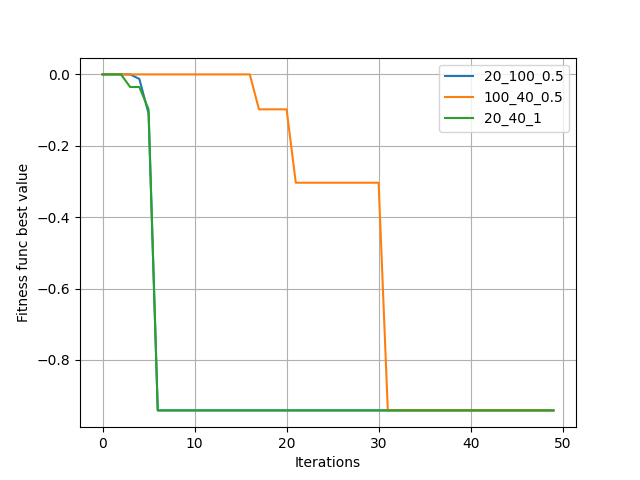
\includegraphics{Easom function.png}
        
        \newpage

        \textbf{six-hump Camel Function} --- відразу знаходить мінімум \\
        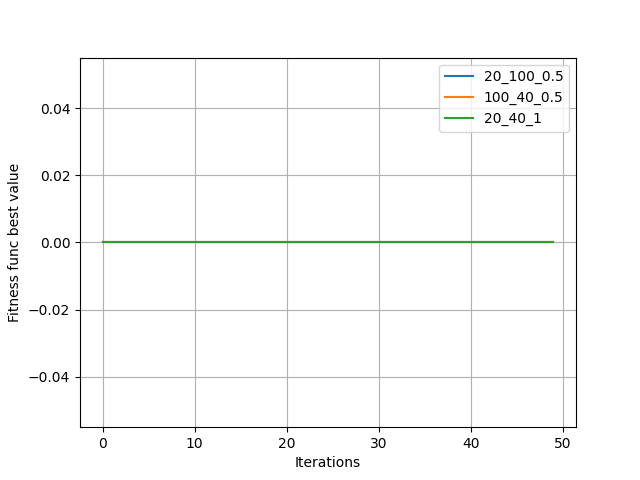
\includegraphics{six-hump Camel function.png}
        
        \newpage

        \textbf{The Goldstein-Price Function} --- відразу знаходить мінімум \\
        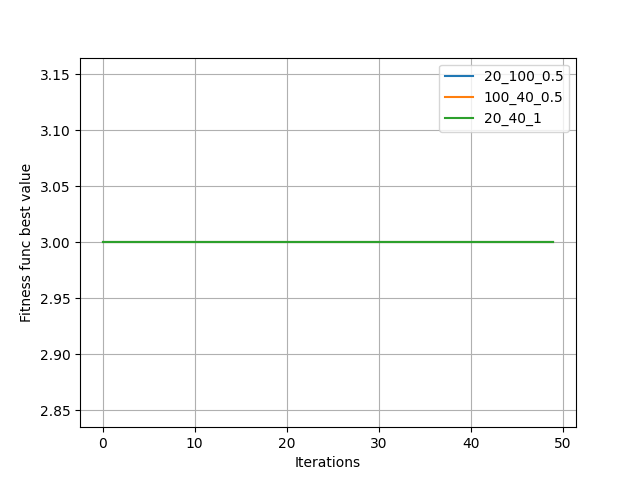
\includegraphics{The Goldstein-Price function.png}

\end{document}